\section{Results at Matched Rate}
\label{sec:results}

Figure~\ref{fig:main} uses validation-selected quantisation; the 0.3\% rate
mismatch slightly favours CRA5. Correctors share an architecture/objective,
with compressor-specific weights. Classical correctors train before quantisation
and evaluate after it; CRA5 uses decoded streams throughout. Quantisation changes
classical corrected nRMSE by 0.07--0.44\%, but the mismatch remains a limitation.

\begin{figure}[t]
\centering
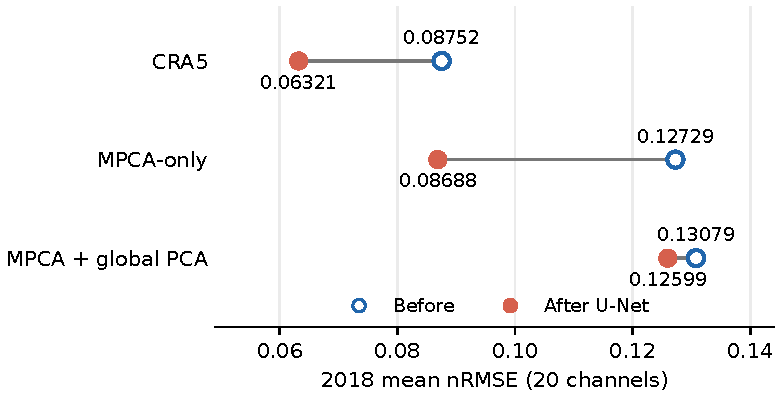
\includegraphics[width=0.90\textwidth]{figs/main_result}
\caption{Matched mean 2018 rates: CRA5 $471.6\times$, MPCA-only $473.1\times$,
and MPCA+global-PCA $472.9\times$. Hollow markers denote baseline and filled
markers add correction without per-frame bits. Values average all 20 channels,
including derived \texttt{tcwv}, matching the 20-channel columns in
Table~\ref{tab:outtime}.}
\label{fig:main}
\end{figure}

CRA5 has lower error before and after correction (Fig.~\ref{fig:main}).
Corrected MPCA-only (0.08688) is only 0.73\% below uncorrected CRA5 (0.08752);
different post-processing prevents a decisive compressor ranking.
At matched rate, global PCA raises corrected error by 45\% versus MPCA-only.

\subsubsection{Decoder-side repair.}
\label{sec:zerobit}
CRA5 direct19 nRMSE falls from 0.08661 to 0.06431
($G=25.8\%$, $\bar G=19.3\%$). With derived \texttt{tcwv}, $G=27.8\%$.

The unchanged bitstream requires no residual side information;
shared correction weights cost about 6.6\,MB in float32 plus inference computation.
This is model-relative predictability, not an information-theoretic bound.
Profiling counts 19.86\,G FLOPs per frame. On an RTX 3080,
float32 GPU-resident inference at batch 8 averages 1.32\,ms per frame with TF32
allowed; this excludes decoder, I/O, and transfer costs.

The 95\% bootstrap intervals for direct19, near and upper $G$ are
[25.32, 26.18]\%, [31.73, 32.62]\% and [3.38, 3.68]\%, respectively. The near-minus-upper difference
is 28.66 percentage points [28.31, 29.01]. Table~\ref{tab:asymmetry} gives group
errors; intervals condition on checkpoint, year and grid.

\subsubsection{Full-year out-of-time evaluation.}
Unlike 2018, the complete 2022 test year is outside CRA5's published training
window. Table~\ref{tab:outtime} shows that the frozen corrector retains its
aggregate improvement: direct-channel $G=26.40\%$ with a 95\% block-bootstrap
interval of [25.90, 26.93]\%. Near-surface gain is 32.79\% [32.28, 33.31]\%
versus 3.60\% [3.46, 3.76]\% aloft, a 9.10-fold ratio.

\begin{table}[t]
\centering
\caption{Full-year CRA5 correction, 1{,}460 frames/year. After$_{20}$ and $G_{20}$
include derived \texttt{tcwv}, matching Fig.~\ref{fig:main}; baseline nRMSE is
0.08752/0.08700 in 2018/2022. All $G$ columns are percentage reductions:
$G_{19}$ excludes \texttt{tcwv}; $G_N,G_U$ use near13/upper6. All checkpoints
are 2017-selected and frozen. Dilated is parameter-matched; Affine is not.}
\label{tab:outtime}
\begin{tabular}{llr@{\hspace{1.5em}}rrrr}
\toprule
Corrector & Year & After$_{20}$ & $G_{20}$ & $G_{19}$ & $G_N$ & $G_U$ \\
\midrule
U-Net & 2018 & 0.06321 & 27.78 & 25.75 & 32.18 & 3.52 \\
 & 2022 & 0.06236 & 28.32 & 26.40 & 32.79 & 3.60 \\
Dilated & 2018 & 0.06354 & 27.40 & 25.38 & 31.61 & 3.82 \\
 & 2022 & 0.06270 & 27.93 & 26.01 & 32.21 & 3.91 \\
Affine & 2018 & 0.08471 & 3.20 & 1.29 & 1.43 & 0.82 \\
 & 2022 & 0.08425 & 3.16 & 1.31 & 1.45 & 0.85 \\
\bottomrule
\end{tabular}
\end{table}

Including derived \texttt{tcwv}, 2022 nRMSE is 0.08700 before and 0.06236 after
correction ($G=28.32\%$); \texttt{tcwv} alone gains 59.43\%. Aggregate gains
do not imply uniform improvement: $v500$ worsens slightly (gain $-0.0082\%$).
